\chapter{Methodology}

\section{Improving the level editor}

To start, it seems reasonable to provide an overview of the unfinished level editor for
InfiniteTux, as wel as some common elements of the game. It is a fair assumption that most
people have played video games are familiar with common enemies in Super Mario Bros., but
InfiniteTux uses open-source assets, so a table of reference has been provided in \autoref{fig:ift-mario}
that maps common components from Super Mario Bros. to their representations in InfiniteTux.

\begin{figure}[h]
    \centering
    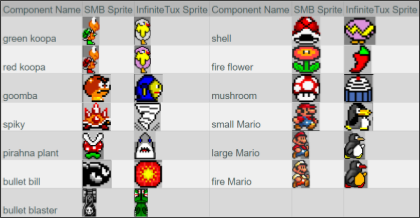
\includegraphics[width=0.8\linewidth]{img/fig10-ift-mario.png}
    \caption{Comparison between \emph{Super Mario Bros.} and \emph{InfiniteTux} components}
    \label{fig:ift-mario}
\end{figure}

The existing interface for the editor is shown in \autoref{fig:ift-editor}. In order to use
this level editor, the user works directly on the blue canvas to place tiles one at a time.
Tiles are selected from the "Tile Picker" panel on the bottom row. The currently selected
tile is shown with a white border in the "Tile Picker" component. The canvas is similar to
a paint application, as the user can draw strokes of tiles to speed up the process. Beside
the "Tile Picker" is a list of checkboxes that indicate the behaviour of the selected tile.
These checkboxes shown the user which tiles contain a powerup, have collision, or are
breakable by the player, all of which is critical information for the level designer. The
last part of the level editor is the top row, which shows the level name, cursor position
in tile coordinates, and has controls for file management.

\begin{figure}[ht]
    \centering
    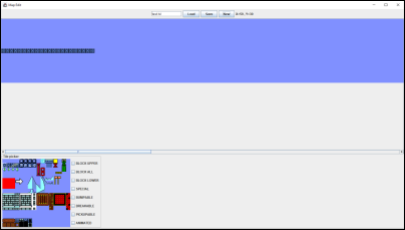
\includegraphics[width=0.8\linewidth]{img/fig11-ift-editor.png}
    \caption{Existing level editor for \emph{InfiniteTux}}
    \label{fig:ift-editor}
\end{figure}

Before starting the implementation of the level editor, it is reasonable to create a list
of desired features based on the usability principles and level editor guidelines that have
been previously mentioned. For each of Rouse's guidelines about level editors, the
functionality that the level editor should support in order to meet the guidelines will be
listed.

\begin{description}
    \item [Guideline 1: The designer should be able to see the world being created while in the process of creating it.] This means that the designer of the level should be able to see the relevant components of the level during its creation. Currently, the tiles of the level are displayed to the user, and the display updates each time the level changes. However, the representation of enemies are missing from this display.
    \item [Guideline 2: Level editors should also provide the designer with extra information about the level, not normally visible in game.] The current level editor lacks this functionality. If working, the "Tile Picker" would show the behaviours of the current tile. However, the behaviours of placed tiles are not shown to the designer at all. Additionally, other important characteristics of the level are not shown, including where Mario initially spawns, as well as the location of the level exit.
    \item [Guideline 3: Level editors should provide the ability to immediately playtest the in-progress level.] The current level editor lacks any in-place level editing capabilities. This could be added by connecting the produced level to the main game. To automate the playtesting process to some degree, an artificial agent could run through the level at each stage where a change happens to check it for playability.
    \item [Guideline 4: A level editor should allow the designer full control over all gameplay critical sections of a level.] The current level editor does not allow the designer to place enemies, change Mario's start position, easily see the behaviour of placed tiles, or even adjust the length of levels.
\end{description}

By comparing the current level editor to Rouse's guidelines, several additions have been
identified: 1) Playtesting should be added. 2) The designer should be able to view tile 
behaviours. 3) The designer should be able to move the level exit. 4) The designer should
be able to place enemies in the level. 5) The resize operation should be supported, so the
user can rapidly adjust the length of the level. Additionally, a few further features should
be added to improve the direct maniuplation task when using the level editor. 6) Undo and
redo for most actions. Addition this list of components to the system will help improve
the overall experience of creating levels.

\section{A suitable level generator for an interactive system}

Several requirements need to be met when building a collaborative level editor. These
requirements include performance, creating levels that are sufficiently different from one
another, and some features that allow for mixed-authorship of levels. Many of the previously
discussed level generators are not suitable for an interactive environment, due to the 
level generation taking a large amount of time. Most levels that would be generated by
evolutionary algorithms fall into this category. Since the set of all possible levels is so
large, finding a satisfactory level through evolving levels takes too long for an
interactive system. One of the gaols of this project is to provide a means for generating
ideas and constructing levels more quickly than by hand. Subsequently, a requirement of the
level generator is that is should produce more intersting ideas than pasting together linear
segments in such a way that InfiniteTux's current level generator (the Notch generator) does
\cite{shaker2016}. To better facilitate mixed-authorship level editing, the leve generator
should also be able to re-generate areas the the user has selected, so that the user and
system can work together toward generating the final level.

The Tanagra level generator creates a rhythm for the level, and the user can modify either
the rhythm or the level geometry to adjust the level to their liking \cite{smith2010}.
Additionally, level segments can be re-generated if the user commands the system. One
drawback to the generation approach taken by Tanagra is that often results in linear levels
where a speedrun playstyle is preferred. There is little to no emphasis on exploration.
However, Tanagra is able to generate levels extremely quickly, due to its use of reactive
grammars and working memory.

Alternatively, occupancy regulated extension (ORE) is abel to produce levels that end up
being less linear than most generators \cite{mawhorter2010, shaker2011}, and can therefore
reward the player for exploration. However, this feature is dependent on a set of chunks 
referred to as the "chunk library", which has to be developed before ORE can produce
any meaningful output. Another drawback is that ORE generation takes longer than Tanagra.
However, ORE does still allow for a collaborator to work on the level concurrently.

Given these considerations, ORE seems like it would be a better fit than Tanagra for the
level generation algorithm for this system. The main advantage of ORE is that it can overlap
partial elvel segments, and supports re-generation. Additionally, a feature that seemed
appealing for a mixed-initiative system was to allow the users of the system to modify the
chunk library that ORE considers. By adding or removing chunks to the library, the user
can gradually tun the created levels to their needs.

In the system, a modified version of ORE was used (mORE). The reason for this is that the 
original ORE generator's source is not readily available, as there was some ambiguity in
the published algorithm, and the chunk library used in the paper was not made publicly
available. However, the approach is still largely based on the ideas or ORE, and pre-authored
chunks are combined in an overlapping manner by anchor points. A few key differences are
worth mentioning, and are detailed in \autoref{table:ore-v-more}. For reference, the mORE
algorithm is described as pseudocode in Appendix A.

\begin{longtblr}[
    caption = {Differences between ORE and mORE},
    label = {table:ore-v-more},
]{|c|X|X|} \hline
    Characteristic & ORE & mORE \\\hline
    Chunk representation & Text file with its own encoding, allowing some extra information like whether a solid tile is part of the ground or a platform. & Text file using the same encoding as InfiniteTux, with the exception of anchors and preserved spaces. \\\hline
    Clipping & Parts of the test chunk that are out of bounds of the level are discarded. & If any part of the test chunk is out of the level, the whole chunk is discarded. \\\hline
    Number of passes & One pass, but extended artificially by the generator adding additional anchor points when it runs out. & Two passes, with two separate sets of chunks working with the same anchors. \\\hline
    Chunk tags & Uses tags for frequency that a particular chunk should be selected. & Uses tags to separate chunk library into first and last sets. \\\hline
    Chunk library & Uses two libraries, one of 22 chunks and one of 20 chunks. & Uses one library of chunks that can be expanded by the user. \\\hline
    Post-processing & Uses post-processing to decorate the level, to fill in areas beneath the ground tiles. It is also used to evenly distribute power-ups across the level. & No post-processing is used. \\\hline
    Running time & 15 seconds for a complete level of 256x15 tiles. & 5 seconds for a complete level of 256x15 tiles. \\\hline
%\end{tabularx}
\end{longtblr}

The chunk library that mORE uses is important, because any content it creates is an
interconnected whole of the chunks in the library. For this project, the chunk library is
not as important as it would be if mORE was not configurable by the user. If the user notices
that some elements that tehy want in their levels are missing, they can always augment the
chunk library to achieve the desired effect. For example, an element not present in mORE's
default chunk library is the pirahna plant. The user could easily draw a plant in the level
canvas and add it to the library, where it would immediately become available for use in the
level generator. The default chunk library is shown in \autoref{fig:more-chunks}. 
Additionaly information that the game and the level generator use is included in the rendering.
For example, the anchor symbol is included, and these points are the anchor points that mORE
uses to connect level segments together. The spaces marked by the word "keep" are 
"preserve points". These are points that are to be kept clear of overlapping geometry. 
Without preserve points,, ceilings could be generated that were lower than three tiles high,
sio that only small Mario can pass, which presents a playability issue, as players that
collected a mushroom power-up may not be able to finish the level. Tiles with a solid red
border on each edge are completely solid, and Mario cannot pass them on any side. Tiles with
a solid border on top are impassable from the top. This particular chunk library is able to
produce levels with branching paths by using chunks with three or more anchor points, with
create a branched path. For example, the first chunk on the third row of \autoref{fig:more-chunks}
contains two points connecting to the ground, and one point on top of a hill. One path can
extend from the ground, and the other from the hill. Most chunks in the library with a single 
anchor point destroy the ability of the algorithm to expand the level, as they take an anchor
without providing any additional points to expand. These chunks are generally marked as
"place last" so that a complete level structure is generated before they are placed. Chunks 
with two anchors often result in a linear section of play.

\begin{figure}[h]
    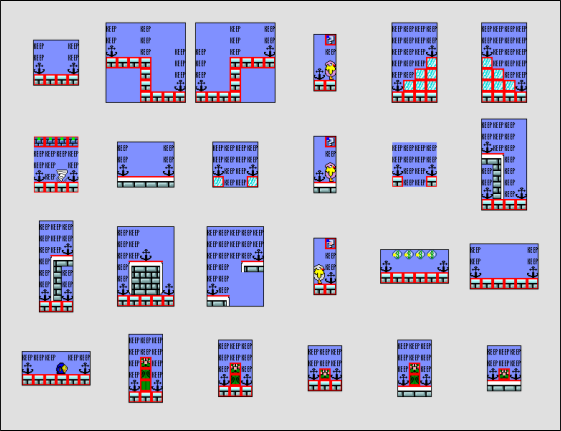
\includegraphics[width=\linewidth]{img/fig12-more-chunks}
    \caption{mORE's default chunk library}
    \label{fig:more-chunks}
\end{figure}

Some sample levels that mORE has generated are shown in \autoref{fig:more-levels}. A
visible issue with the generator is that it produces that look incomplete. Where hills are
drawn, only the hilltops shown. The lowermost point of ground has an unsightly gap between
it and the bottom of the screen. However, these omissions are purely cosmetic and do not
affect the gameplay of the level. The default generator of InfiniteTux, the Notch generator,
addresses these issues with a function that identifies these gaps as they are built. If
mORE were to resolve the issue, it would require a post-processing step to identify and fix
the problem areas. In each of the sampled levels, sections of non-linear play occur in a few
spots, so the player can make a choice about which path the want to take to reach the end. 
This effect is not nearly as common in the Notch generator, except for the occasional hill
that the player can leap on for some reward.

\begin{figure}[h]
    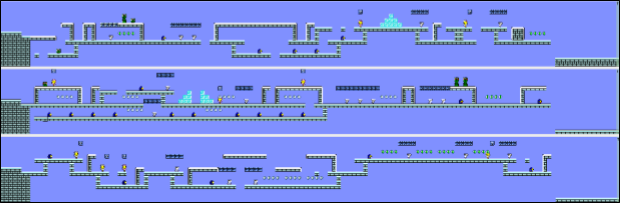
\includegraphics[width=\linewidth]{img/fig13-more-levels.png}
    \caption{three levels generated using mORE}
    \label{fig:more-levels}
\end{figure}

\section{Adding collaborative elements to level creation}

So far, a level generation algorithm and general improvements to the existing level editor
interface have been covered. However, the system as currently specified sites in the 
family of low-initiative systems. The system does not provide much in terms of feedback on
the user's design, or notify the user of constraints that are important in generating 
2D-levels, such as whether or not the user can actually complete the level.

To address the first issue, a section of the interface was created that shows the user
information about both level pacing and a player's solution to a level. In many games,
a higher enemy density indicates a higher level difficulty, as enemies present a dynamic
challenge that the player must actively avoid. At the same time, the presence of power-ups
will reduce the difficulty of a level. Power-ups and rewards are also often used as
incentives for player exploration. Often, Mario levels are too large to fit on a single 
screen, and it may be difficult for the designer to quickly get an overview of the
distribution of enemies and rewards. To address this issue, a time series is shown to the
user that can provide a quick overview of the density of enemies and rewards across a
level. At each tile, the number of enemies or rewards is recorded, and this is shown on
the time series. The time series provides the designer with a way of visualising how
spread out the rewards and enemies on a level are. Using this information, the designer can
recognize issues with level pacing and course-correct the level.

The second issue, playability, is much harder to account for. Since most platformer games
use continuous phsics, it is difficult to construct a level in a random way while ensuring
playability \cite{smith2010}. Tanagra is able to solve this problem by using linear chunks 
and ensuring that adjacent chunks in a level line up, such that the start and end tiles
match neighbouring chunks. However, when considering the entire space of possible Mario
levels, levels must exist where neighbouring chunks do not line up. As such, this seems to
be an arbitrary restriction to make sure that generated levels are always playable, but it
comes at the cost of reducing the space of generated levels. Sorenson and Pasquier's
generator, or generators like \emph{FUN Pledge} enforce level playability by using a ballistic
model for jumps. However, since mORE is based on ORE< none of these approaches are feasible.

In order to ensure level playability, a level playthrough is simulated with an A-star agent.
The particular agent that was implemented was chosen since it won the MarioAI competition,
is performant, and uses a similar level representation, so it could be integrated easily.
The agents of the MarioAI competition are guaranteed to select an action within a single 
frame. Additionally, the agent can run at an uncapped framerate, and on a background thread
from the level editor user interface. By taking advantage of these features, the agent was
able to be incorporated directly into the level editing process. Each time th user makes
a change to the level, the agent is called to simulate playing the level. This performs fairly
well, and in most cases returns results in a few seconds on a computer with a 6-core, 3.6 GHz
processor. The results of the agent's test run are returned to the user in two different
ways. First, if the agent was not able to clear the level, it may imply that the level is
not possible. The x-coordinate of the furthest point the agent was able to reach is displayed
to the user as an error message. Changes that result in the level being successfully cleared
also clear the message. Additionally, a trace of the agent playing the level is created on a
time series. At each frame while playing the level, the agent's inputs are recorded. This
data is shown as a series of labelled block functions for each action. From this data, the
user can roughly estimate the pacing of the level as time progresses. Sections on the graph
where the only actions are left and speed probably indicate that the sections are easy. On
the other hand, constant breaks in the rhythm, times where the agent had to let go of speed,
or move backward, indicate that the level is more complex, or that elements in the level are
causing slowdown to occur, but the system's plot doesn't offer any information on the source
of the effect.

One notable feature is the undo operation, which also applies to the system's actions. If
the designer does not approve of system changes, they can undo the operation quickly, and try
to generate it again.

A collaborative feature of the level editor that has yet to be mentioned is the user's direct
access to the underlying chunk library that mORE uses in its level generation. The user is 
able to directly create a new chunk for the library by drawing it on the level canvas and
clicking a button in the interface. The chunk immediately appears in a separate panel, with
the other chunks that the system uses. The users can modify the library by deleting or tagging
chunks. A tag is a rule that the level generator uses during level generation. The only tag
currently available is "place last" which can be used to force the tagged chunk to only
be considered for placement after the first set of chunks is placed.


\section{Final system}

The final interface for the system is presented in \autoref{fig:final-system-overview} and
\autoref{fig:chunk-library}. A typical workflow would be to first have the system generate
a level. After generating the level, the designer consults any error messages and revises
the level until it is playable. Optionally, the designer may consult the component distribution
or the agent's most recent level trace to determine whether or not the level is appropriately
paced. The designer may also edit the library the generator is using during their session,
and re-generate parts of the level as they proceed. Additionally, the designer may playtest
the level at any point to come to their own conclusions about the suitability of the level.

\begin{figure}[h]
    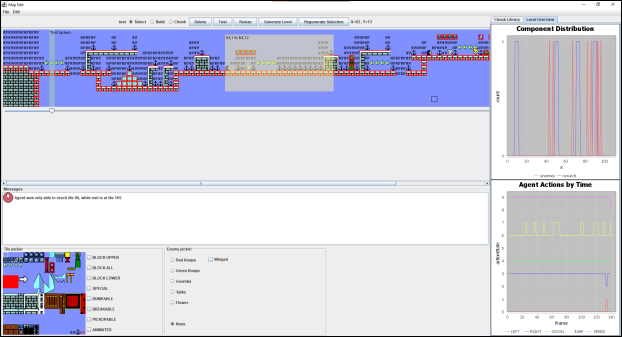
\includegraphics[width=\linewidth]{img/fig14-final-system-overview.png}
    \caption{Final system with "Level Overview" panel open}
    \label{fig:final-system-overview}
\end{figure}

\begin{figure}[h]
    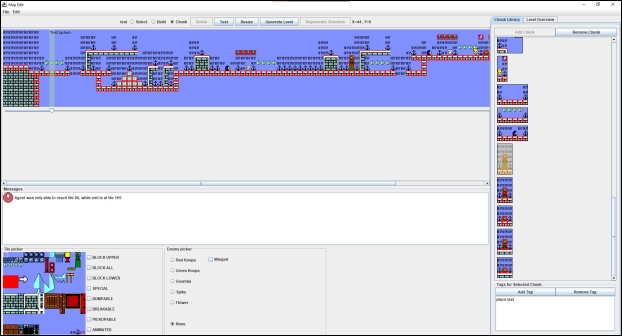
\includegraphics[width=\linewidth]{img/fig15-chunk-library.png}
    \caption{Final system with "Chunk Library" panel open}
    \label{fig:chunk-library}
\end{figure}